\begin{figure}[h!]
\textbf{Tema d'Esame di Gennaio 2016}\\ \\
 Prima di chiudere l'interruttore $S1$, la tensione ai capi del condensatore $C1$ è pari a $12V$. Determinare quanto tempo deve passare dalla chiusura dell'interruttore $S1$ perché la corrente
che scorre in $R2$ diventi inferiore a $10 \mu A$. $R1=R2=2k\Omega$. $C1=1\mu F$.
	\begin{center}
		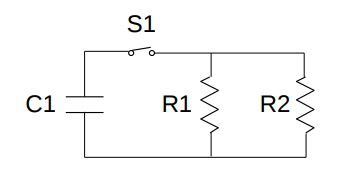
\includegraphics[scale=0.8]{ES5/GEN052016.jpg}
	\end{center}
\end{figure}

\begin{figure}[h!]
\textbf{Tema d'Esame di Febbraio 2016}\\ \\
Si determini la differenza di potenziale ai capi della resistenza $R4$ del circuito mostrato in figura. La differenza di potenziale fornita dalla batteria è di $12V$ e i valori delle resistenze sono rispettivamente $R2=15\Omega, R3=40\Omega,R4=25\Omega, R5=R6=32\Omega, R1=R7=18\Omega$
	\begin{center}
		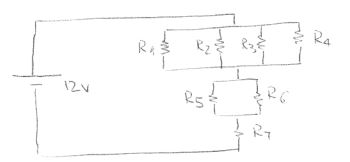
\includegraphics[scale=1.1]{ES5/FEB052016.jpg}
	\end{center}
	\noindent\fbox{
		\parbox{\textwidth}{
			\null\hfill \textbf{Soluzione:} $V_4 = 1.60 V$\\
			\textbf{Procedimento: } \\
			Semplificazione delle Resistenze:\\
			
			$R_{1234}=\frac{1}{\frac{1}{R_1}+\frac{1}{R_2}+\frac{1}{R_3}+\frac{1}{R_4}}=\frac{1}{\frac{1}{18\Omega}+\frac{1}{15\Omega}+\frac{1}{40\Omega}+\frac{1}{25\Omega}}=5.34\Omega$\\ \\ 
			$R_{56}=\frac{R_5\cdot R_6}{R_5+R_6}=\frac{32\Omega\cdot 32\Omega}{32\Omega+32\Omega}=16\Omega$\\ 
			$R_{tot}=R_{1234}+R_{56}+R_7=5.34\Omega+16\Omega+18\Omega=39.34\Omega$\\
			Ricordando che la tensione in parallelo non cambia, così come non cambia la corrente in serie:\\
			$I_{tot}=I_{1234}=I_{56}=I_7=\frac{V}{R_{tot}}=\frac{12V}{39.34\Omega}=0.30A$\\
			$V_4=V_1=V_2=V_3=R_{1234}\cdot I_{tot}=5.34\Omega\cdot 0.30A=1.60V$
		}
	}	
	
\end{figure}

\begin{figure}[h!]
\textbf{Tema d'Esame di Giugno 2016}\\ \\
Se il generatore fornisce una differenza di potenziale di $12 V$, qual'è la caduta di potenziale ai capi della resistenza $R5$. Si considerino le resistenze 
$R1= 35 \Omega, R2= 10 \Omega, R3= 24 \Omega, R4= 18 \Omega, R5= 30 \Omega, R6= 21 \Omega, R7=17 \Omega , R8=19 \Omega$.
	\begin{center}
		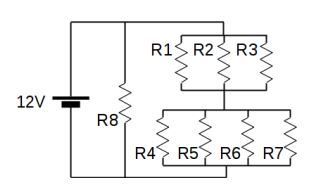
\includegraphics[scale=1]{ES5/GIU052016.jpg}
	\end{center}
	\noindent\fbox{
		\parbox{\textwidth}{
			\null\hfill \textbf{Soluzione:} $V_5 = 5.60 V$\\
			\textbf{Procedimento: } \\
			Semplificazione delle Resistenze:\\
			$R_{123}=\frac{1}{\frac{1}{R_1}+\frac{1}{R_2}+\frac{1}{R_3}}=\frac{1}{\frac{1}{35\Omega}+\frac{1}{10\Omega}+\frac{1}{24\Omega}}=5.87\Omega$\\ \\ 
			$R_{4567}=\frac{1}{\frac{1}{R_4}+\frac{1}{R_5}+\frac{1}{R_6}+\frac{1}{R_7}}=\frac{1}{\frac{1}{18\Omega}+\frac{1}{30\Omega}+\frac{1}{21\Omega}+\frac{1}{17\Omega}}=5.12\Omega$\\
			$R_{tot}=\frac{R_{1234567}\cdot R_8}{R_{1234567}+ R_8}=6.96\Omega$\\
			Ricordando che la tensione in parallelo non cambia, così come non cambia la corrente in serie:\\
			$I_{1234567}=\frac{V}{R_{1234567}}=\frac{12V}{10.98\Omega}=1.09A$\\
			$V_5=V_4=V_6=V_7=R_{4567}\cdot I_{1234567}=5.12\Omega\cdot 1.09A=5.60V$
		}
	}	
	
\end{figure}

\begin{figure}[h!]
\textbf{Tema d'Esame di Luglio 2016}\\ \\
Nel circuito in figura, la corrente attraverso $R6$ è $i_6=1.2 A$ e le resistenze sono $R1=R2=R3=4.0 \Omega, R4= 10 \Omega, R5= 4.0 \Omega , R6= 2.0 \Omega$. Qual'è la forza elettromotrice della batteria (ideale)?
	\begin{center}
		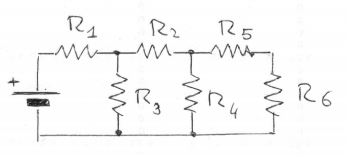
\includegraphics[scale=0.8]{ES5/LUG052016.jpg}
	\end{center}
	\noindent\fbox{
		\parbox{\textwidth}{
			\null\hfill \textbf{Soluzione:} $V = 37.445 V$\\
			\textbf{Procedimento: } \\
			Ricordando che la tensione in parallelo non cambia, così come non cambia la corrente in serie proseguiamo semplificando le resistenze e aggiornando man mano corrente e tensione:\\
			$R_{56}=R_5 + R_6=4\Omega + 2\Omega=6\Omega$\\
			$V_{56}=R_{56}\cdot I_{56}=6\Omega\cdot 1.2A=7.2V$\\\\
			$R_{456}=\frac{R_{56}\cdot R_4}{R_{56}+R_4}=\frac{6\Omega\cdot 10\Omega}{6\Omega + 10\Omega}=3.75\Omega$\\
			$I_{456}=\frac{V_{56}}{R_{456}}=\frac{7.2V}{3.75\Omega}=1.92A$\\ \\
			$R_{2456}=R_2+R_{456}=4\Omega+3.75\Omega=7.75\Omega$\\
			$V_{2456}=R_{2456}\cdot I_{456}=7.75\cdot 1.92A=14.88V$\\ \\
			$R_{23456}=\frac{R_3\cdot R_{2456}}{R_3+ R_{2456}}=\frac{4\Omega \cdot 7.75\Omega}{4\Omega+ 7.75\Omega}=2.64\Omega$\\ \\
			$I_{23456}=I_{tot}=\frac{V_{23456}}{R_{23456}}=\frac{14.88V}{2.64\Omega}=5.64A$\\
			$R_{tot}=R_1+R_{23456}=4\Omega+2.64\Omega=6.64\Omega$\\
			$V=R_{tot}\cdot I_{tot}=6.64\Omega \cdot 5.64A=37.45V$
		}
	}	
	
\end{figure}